\documentclass[binding=0.6cm,LaM,english,noexaminfo,oneside]{sapthesis} % LaM for a Laurea Magistrale
\usepackage{microtype}
\usepackage{babel}
\usepackage[utf8]{inputenx}
\usepackage{hyperref}
\usepackage{tabularx}
\usepackage{listings}
\usepackage{xcolor}

\definecolor{ao}{rgb}{0.0, 0.5, 0.0}

\lstset{
    language=C++,
    frame=tb, % draw a frame at the top and bottom of the code block
    tabsize=4, % tab space width
    showstringspaces=false, % don't mark spaces in strings
    numbers=left, % display line numbers on the left
    commentstyle=\color{ao}, % comment color
    keywordstyle=\color{blue}, % keyword color
    stringstyle=\color{red}, % string color
    basicstyle=\footnotesize\ttfamily,
    basewidth = {.48em}
}

\usepackage[backend=bibtex]{biblatex}
\bibliography{biblio.bib}

\setlength{\parindent}{4em}
\renewcommand{\baselinestretch}{1.5}

\hypersetup{pdftitle={My thesis},pdfauthor={Francesco Biccari}}
\title{BlueTracer: \\ a Robust API Tracer for Evasive Malware}
\author{Simone Nicchi}
\IDnumber{1705157}
\course{Master of Science}
\courseorganizer{Faculty of Information Engineering, Informatics and Statistics}
\AcademicYear{2017/2018}
\copyyear{2018}
\advisor{Prof. Camil Demetrescu}
\coadvisor{Dr. Daniele Cono D'Elia}
\coadvisor{Dr. Emilio Coppa}
\authoremail{nicchi.1705157@studenti.uniroma1.it}
\begin{document}
\frontmatter
\maketitle
\dedication{Ai miei genitori, che non hanno mai smesso di supportarmi}

\begingroup
\clearpage% Manually insert \clearpage
\let\clearpage\relax% Remove \clearpage functionality
\vspace*{-2cm}% Insert needed vertical retraction
\begin{abstract}

\iffalse
Malwares are a threat

Dynamic analysis is favoured over static analysis

One dynamic analysis technique is API hooking/tracing

Malwares are also evasive

Problem: API hooking and tracing evasive samples

Solution BlueTracer
\fi

Malicious software (or malware) is any software specifically designed to bring harm to a computer system. The problem posed by malwares is one which is becoming increasingly important, as new and more sophisticated malwares arise every day and the economical damage for organizations keeps worsening \cite{Cisco}. To face this threat, professionals are typically aided by a range of automatic tools capable of analysing and detecting malicious software.

Malware analysis can be carried out either statically or dynamically. Dynamic analysis encompasses techniques that execute a sample and observe the actions it actually performs, whereas in static analysis the sample is examined without running it. Such techniques have evolved over time to keep track with the increasing complexity and diversity of malwares. However, in recent years, the shift towards automation, caused by the need of dealing with a huge and ever-growing number of samples, together with the rising complexity of obfuscation mechanisms utilized by malwares, has strongly favoured dynamic analysis.  

One of the most employed dynamic analysis techniques is function call monitoring. Generally, a function is made up of code which carries out a particular task, like for example creating a file or printing a message. Although the utilization of functions allows for easy re-usability of code and simpler maintenance, the propriety which makes them particularly valuable from a program analysis perspective is that they abstract the implementation details, providing a semantically richer representation of some functionality. For instance, let us consider a sorting function; it might not be important to know the underlying sorting algorithm as long as it is known that the function sorts the input number set. In the context of dynamic analysis, the abstractions provided by API calls and system calls (or eventually Windows Native APIs) are incredibly helpful since they can be used to grasp the overall behaviour of the sample being analyzed.

The typical technique used for function calls monitoring in dynamic malware analysis is \textit{API hooking}, i.e. the interception of function calls provided by DLLs. The idea is to alter the original sample so that, besides the function of interest, a \textit{hooking} function is also called, which is in charge of performing the wanted analysis, e.g. logging the function invocation on a file or analyzing the function's parameters \cite{Egele:2008:SAD:2089125.2089126}.      

A problem that all dynamic analysis techniques have to face, including function call monitoring by means of API hooking, is the widespread of evasive malwares. Such malwares check whether or not they are being executed in an adverse environment and conceal their harmful behaviours accordingly, like for example by carrying out an exit sequence \cite{BluePill}. Unfortunately, such anti-evasion mechanisms are frequently adopted my malicious samples. According to Symantec's Internet Security Report of March 2018, 18\% of new malware were virtual-machine-aware \cite{Symantec}. To make matters worse, the API hooking techniques presented in literature are easily detectable and are not coupled by any mechanism to hide their presence from evasive malwares.

The goal of this thesis is to present \textbf{BlueTracer}, a robust library and system call tracer for Windows applications, specialized in the monitoring of evasive malwares. BlueTracer is based on the Intel Pin \cite{Pin} dynamic binary instrumentation (DBI) framework and is able to counteract malwares' anti-evasion measures thanks to its integration with BluePill, a software toolkit built on top of a DBI layer which allows the simulation of the execution environment a particular malware was designed for and conceals any virtualization artifacts and setup details which might set off evasion \cite{BluePill}. BlueTracer is capable of tracing the input values, the output values and the return values of an extremely wide range of system calls (including Windows Native APIs) and API calls. Moreover, it also supports the tracing of Windows callbacks functions and Windows asynchronous procedure calls (APC). To tool was tested on a benign application aimed at assessing how good an anti-malware system is against evasion techniques and on actual evasive malwares, proving to be effective in both tracing the samples' activity and remaining undetected.                
\\
\textbf{Thesis Structure}. The remaining part of this thesis is structured as follows.
Chapter 1 describes the major \textit{API hooking} techniques present in literature, outlining their stengths and weaknesses, especially from a detection point of view. \\
Chapter 2 introduces the concept of Dynamic Binary Instrumentation (DBI) and presents Intel Pin, the framework used to develop BlueTracer. \\
Chapter 3 focuses on the implementation of the tool, on its structure and the design choices which were made during its development. \\
Chapter 4 illustrates the experimental results and assesses the tool's effectiveness. \\
Finally, in Chapter 5, conclusions are presented, together with possible future developments.     

\end{abstract}
\endgroup

\tableofcontents

\mainmatter
\chapter{API Hooking: State of The Art}
In literature there are many different implementations of API hooking. The objective of this chapter is to provide an outline of the various approaches utilized to hook functions in DLLs, outlining the benefits and the limitations of each technique, with a strong focus on their detection by malicious software. In particular, the focus will be on user space API hooking of \texttt{Win32} binaries, since this is BlueTracer's current field of application. Obviously, as it is the norm in malware analysis, it also assumed that the program under study is only available in binary form.

Depending on their underlying implementation, API hooking techniques can be divided in three broad categories: \textbf{Binary Rewriting Based}, \textbf{Virtul Machine Introspection (VMI) Based} and \textbf{Dynamic Binary Instrumentation (DBI) based}.   

\iffalse
backmatter turns off chapter numbering
\fi
\begin{section}{Binary Rewriting Based Hooking}

Binary rewriting based hooking involves inserting hooks at the API entries, via one of the following two approaches:
\begin{enumerate}
\item Redirecting all \texttt{call} instructions so that the hook is called instead of the original function.
\item Rewriting the function of interest such that, before its invocation, the hook is executed. 
\end{enumerate} 

In both cases the hook function gains access to all the arguments present on the stack, thus being able to carry out all the required analysis operations.

The main techniques which use the first approach are \textit{Import Address Table (IAT) Patching}, \textit{Export Address Table (EAT) patching} and \textit{Proxy DLL}. On the other hand, the most significant techniques which use the second approach are \textit{inline hooking} and \textit{debugger based hooking} (\textit{Figure 1.1}).



\begin{figure}[h]
\centering
\hspace*{-3em}
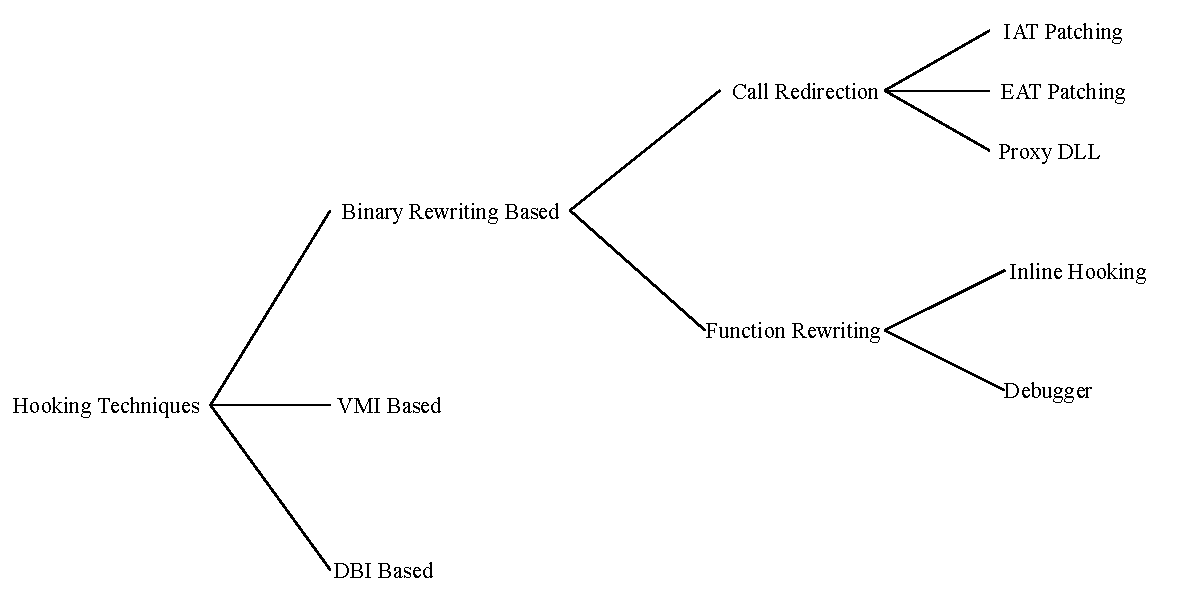
\includegraphics[scale=0.8]{Figures/API-hooking-3.pdf}
\caption{\textit{API hooking techniques classification}}
\end{figure}

\subsection{Import Address Table (IAT) patching}

In the header of every Portable Executable (PE) file there is an Import Address Table (IAT) for every dynamic-link library (DLL) that is included by the executable \cite{Berdajs:2010:EAU:1815744.1815746} (\textit{Figure 1.3}). This table is utilized to indicate the location of DLL-imported functions in virtual memory and is filled by the Windows loader with the actual function memory addresses after the executable is loaded in memory.

\begin{figure}[h]
\centering
\hspace*{-3em}
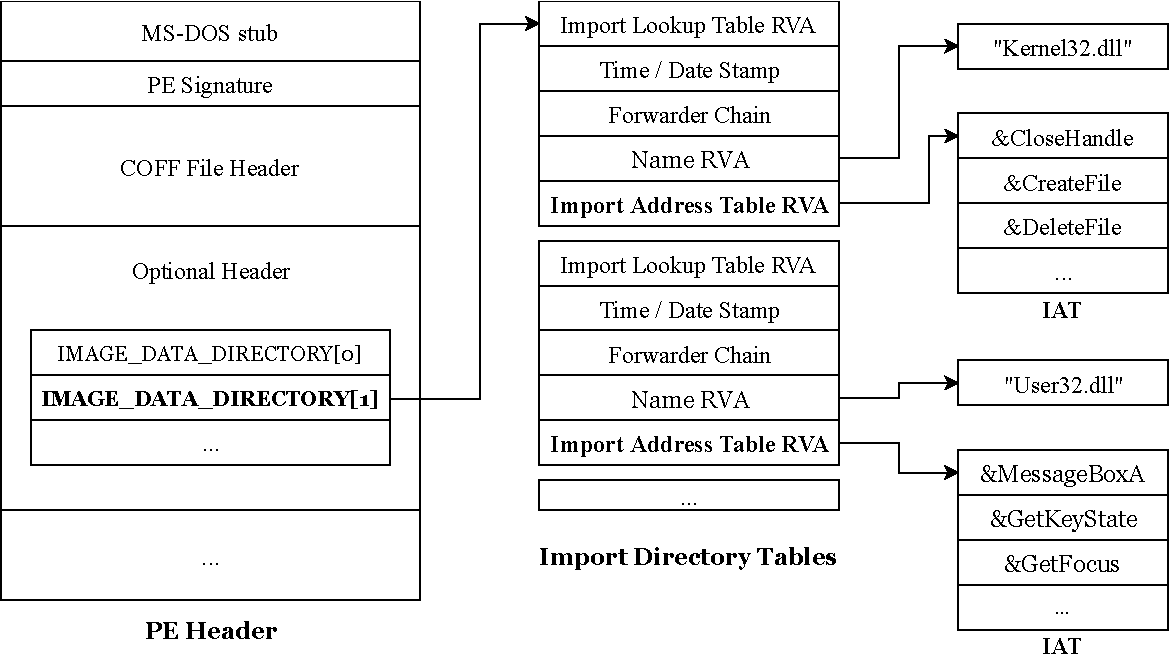
\includegraphics[scale=0.8]{Figures/IAT-3.pdf}
\caption{\textit{IAT in PE header}}
\end{figure}

The idea is to overwrite the original pointer to an imported API function so that, instead of pointing to the original API, it will point to a different function.

\newpage

Despite being extremely simple to implement, IAT patching suffers from a couple of disadvantages, which significantly limit its use in practice:
\begin{itemize}
    \item It is incredibly easy to detect by simply examining the entries of the IAT and checking whether or not each address falls inside the memory range of the DLL that should contain the function \cite{HookingDetection}.
    \item It is ineffective when function pointers are acquired dynamically, e.g. via \texttt{LoadLibrary} and \texttt{GetProcAddress} \cite{Buescher:2011:BIS:2186328.2186347}.
\end{itemize}

\subsection{Export Address Table (EAT) patching}

Export Address Table (EAT) patching is similar to IAT patching, with the difference that DLL export address tables are patched instead. The export address table (EAT) contains the name of every function exported by the DLL together with the relative virtual address (RVA) where the function can be found, which is relative to the DLL base address when loaded in memory. To hook an API function via EAT patching all that is needed is to overwrite the corresponding address in the table with the address of another function.

EAT patching produces similar results to the ones obtained through IAT patching, but, unlike IAT patching, the created hooks are global, i.e. they affect every program which utilizes the altered DLL \cite{Berdajs:2010:EAU:1815744.1815746}.

However, in a similar manner to what occurs for IAT patching, it can be easily detected to by simply examining the entries of the EAT and checking whether or not each RVA, when added to the DLL base address, falls within the DLL memory range \cite{Stuttard:2014:ADC:2616217}.

\subsection{Proxy DLL}

In the Proxy DLL approach to hooking, also known as Trojan DLL, the DLL containing the functions to be hooked is replaced with another one having an identical name and exporting all the symbols of the original DLL \cite{CodeProjectHooking}. In addition to calling the original functions so that they can carry out their tasks, the Proxy DLL may also make available different implementations for the hooked functions \cite{Berdajs:2010:EAU:1815744.1815746}.

Even though a Proxy DLL is trivial to implement, it is also extremely easy to detect since the original DLL is substituted with another file, which is very likely to have a different size. Moreover, checksums could be employed to detect the presence of a Trojan DLL.


\subsection{Inline hooking}

In \textit{inline hooking} the API to be hooked has its initial instructions (at least the first 5 bytes) overwritten with an unconditional jump to a replacement function. In order to ensure that the API's original functionality is not lost due to the modification of its entry point, a \textit{trampoline function} is created, consisting of a copy of the overwritten instructions and an unconditional jump back to the unaltered portion of the original function. As a result of this, the replacement function can invoke the original function by calling the trampoline, after performing all the desired analysis operations \cite{Berdajs:2010:EAU:1815744.1815746}.
\textit{Figure 4} illustrates a program's execution flow before and after the use of \textit{inline hooking}.

\begin{figure}[h]
\centering
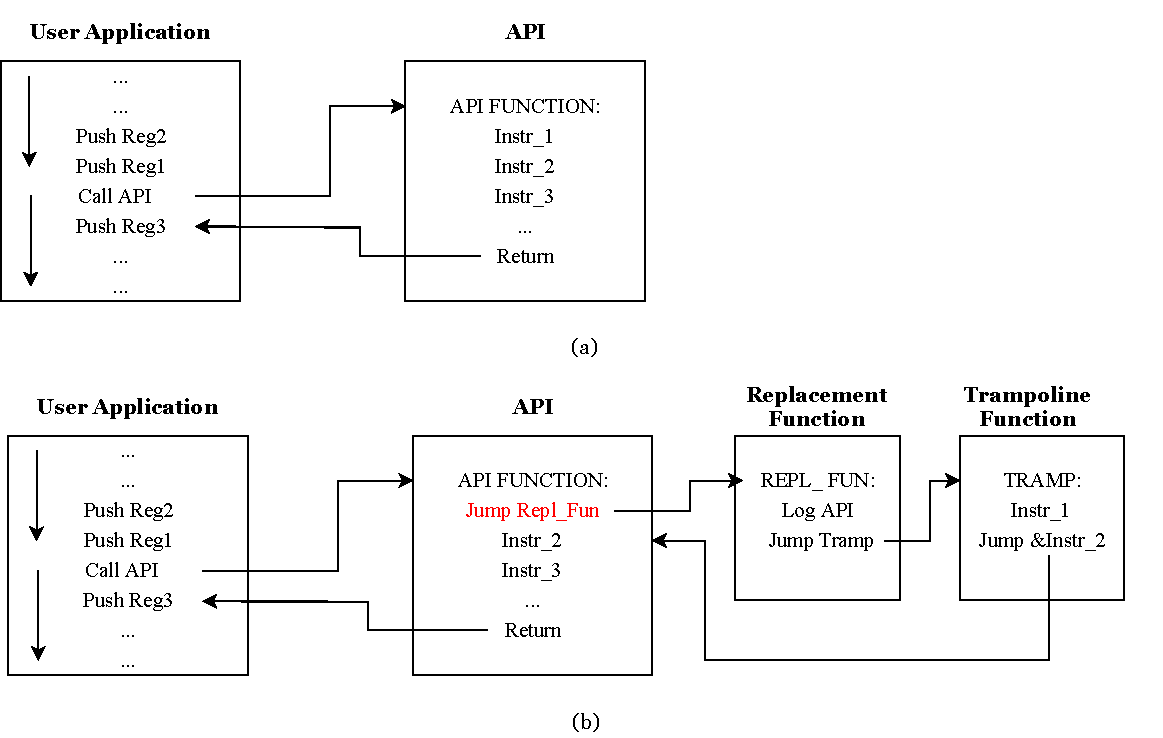
\includegraphics[scale=0.8]{Figures/Inline.pdf}
\caption{\textit{(a) Ordinary API call execution flow \\
				  (b) API call with inline hooking}}
\end{figure}

\newpage

\textit{Inline Hooking}, which was made famous by its employment  in the Microsoft \textit{Detours} Windows API hooking library, is one of the most used API hooking techniques since it offers a number of advantages:
\begin{itemize}
\item It is fast and efficient.
\item It can be utilized to hook any code, not just operating systems APIs, but also programmer defined functions \cite{Rootkit}. 
\item Unlike IAT patching, the type of command used to call the function does not matter, meaning that the hooking will be effective regardless of the fact that a function is called using the IAT or using \texttt{LoadLibrary} together with \texttt{GetProcAddress}.
\end{itemize} 

Unfortunately though, \textit{inline hooking} is also affected by some limitations:

\begin{itemize}
\item Can be easily detected, for instance by comparing the code section of system libraries in memory with a matching original copy loaded from the file system to detect library modifications \cite{Buescher:2011:BIS:2186328.2186347} or by searching API entry points for specific patterns (e.g. presence of \texttt{jmp} instructions) \cite{HookingDetection}.
\item It needs additional modifications in the case where the function's entry points includes specific instructions, like ones which contain relative memory addresses. In fact, such instructions cannot be executed from a trampoline as the trampoline is located in a different memory location than the one of the original program code \cite{Berdajs:2010:EAU:1815744.1815746}.
\end{itemize}

\subsection{Debugger Based Hooking}

Hooking through the use of a debugger is realized by instructing the debugger to position a breakpoint at the entry point of the target API function. The placement of a breakpoint involves overwriting the initial instructions of the target API functions with CPU specific instructions, like \texttt{INT 3} for \texttt{IA-32}. These lead the CPU to throw a debug exception in case they are pointed by the current instruction pointer (IP). The exception is then intercepted by the debugger, which is able to deduce the API which is being called by the application from the address at which the exception took place \cite{HookingDetection}. Moreover, the debugger also has total control over the memory contents and the CPU state of the process being debugged.

Contrarily to inline hooking, a debugger can be used to hook functions whose entry points include instructions containing relative addresses \cite{Berdajs:2010:EAU:1815744.1815746}.

On the other hand, a debugger is much easier to detect. In fact, there exist specific Windows APIs whose purpose is to find out whether or not the current process is being debugged. For example, \texttt{IsDebuggerPresent} allows to determine if the calling process is running under a debugger, while \texttt{CheckRemoteDebuggerPresent} checks for the presence of a debugger in a separate process. 
In addition, the \texttt{INT 3} instruction in an API entry point immediately gives away the debugger's presence \cite{HookingDetection}.
\end{section}

\begin{section}{Virtual Machine Introspection (VMI) \\ 
Based Hooking}

Virtual Machine Introspection (VMI) based hooking relies on the idea of executing the target program in an emulated environment, typically with QEMU being used as virtual machine monitor (VMM). Function calls are monitored by comparing the virtual processor's instruction pointer with the RVAs of DLLs' exported functions when added to the DLL base address. Function arguments are also monitored and this is done by providing them to callback routines, which perform the appropriate tracking operations.

In theory, a PC emulator allows to have functionalities similar to the ones of a debugger, i.e. the code being monitored can be stopped at any arbitrary point during its execution, allowing its registers and virtual memory to be inspected, with the added advantage of not being subject to the aforementioned issues related to breakpoints.
Moreover, VMI based hooking is harder to detect with respect to the previously illustrated hooking techniques, since emulation is utilized to execute an unknown binary with a complete operating system in software, without the sample being never ran directly on the processor \cite{Bayer2005TTAnalyzeA}.

The significant drawback of VMI based hooking is that it incurs in the \textit{semantic gap} problem, i.e. the issue of deducing high-level information from the raw system information by making sense of the CPU state and memory contents \cite{Egele:2008:SAD:2089125.2089126}. VMI based hooking tools
might need an in-depth knowledge of kernel data structures or other details at low-level, which could constitute a complication when dealing with proprietary operating systems. For this reason, as of right now, VMI is not as effective in practice as a traditional debugger when investigating a sample.

\end{section}

\begin{section}{Dynamic Binary Instrumentation (DBI) \\
Based Hooking}

Dynamic Binary Instrumentation (DBI) is an analysis technique in which the behavior of a binary application is inspected at run-time via the injection of instrumentation code. Such code, after being injected, executes as a component of the ordinary instruction flow, allowing to learn information about the behavior and the state of a sample at different points during its execution \cite{DBI}. In DBI based hooking, the learnt information refers to which APIs are called and, possibly, with which arguments and return values. 

There indeed exist DBI based API tracing tools that rely on the previously illustrated idea, namely \textit{drstrace} and \textit{drltrace}, which are both built on top of the DynamoRIO \cite{DynamoRIO} DBI framework. In particular, \textit{drstrace} is a system call tracer for Windows, while \textit{drltrace} is an API calls tracer for both Windows and Linux applications. These tools, however suffer from two notable drawbacks:

\begin{itemize}
\item They are not equipped with any mechanism aimed at cloaking the execution environment in order to prevent a malicious sample from detecting the DBI.
\item They are limited in the amount of information recorded relative to the traced APIs. This applies particularly to \textit{drltace}, which, unlike \textit{drstrace}, does not log return values and output values for arguments, in addition to not providing a mechanism for translating enumerations' constants to the appropriate name. Furthermore, both tools do not take into consideration Windows callbacks and asynchronous procedure calls (APC).
\end{itemize}

\end{section}

\begin{section}{Conclusion}

In this chapter it was shown how the state of the art API hooking techniques suffer from a number of remarkable shortcomings, especially when dealing with evasive malwares. In fact, binary rewriting based hooking techniques are all easily detectable, while VMI, although harder to uncover, is affected by the \textit{semantic gap problem}. Finally, existing DBI based API tracing tools are not accompanied by adequate cloaking mechanisms and are limited in the amount of logged information. The aforementioned issues indicate that there is a need for a robust API tracer, specialized in the analysis of evasive malwares and with extensive logging capabilites. This is the rationale at the heart of BlueTracer. 

\end{section}

\cleardoublepage
\phantomsection % Give this command only if hyperref is loaded

\chapter{Dynamic Binary Instrumentation and Intel Pin}

\chapter{Implementation}
In this chapter BlueTracer's implementation will be discussed, providing a detailed account on how the tool is organized, on the design choices which were made during its development process, on how encountered challenges were dealt with and on the decisions which were taken to improve performance.

BlueTracer, being a part of Blue Pill, is also implemented using Pin, a dynamic binary instrumentation framework by Intel, which is vastly utilized for program analysis, testing of software and in the security field. The version of Pin used for the development of the tool is 3.5, in order to benefit from the notable improvements, both in terms of execution speed and offered features, which were introduced going from the 2.14 release to the 3.x series. Pin comes with its own OS-agnostic and compiler-agnostic runtime, called PinCRT. PinCRT exposes three layers: a generic operating system interface providing basic OS services (e.g. process and thread control), together with C and C++03 (without RTTI) runtime layers, for writing instrumentation and analysis routines \cite{Pin}.   

BlueTracer has been organized primarily taking into account the rich set of APIs offered by Pin, which have led to the decision to split the tool in three parts: the first aimed at \textbf{native APIs tracing}, the second for \textbf{APIs tracing} and the last focused on \textbf{callbacks and APCs tracing} (\textit{Figure 3.1}). In particular, the tracing of native APIs also employs a different source of API information (\textit{Dr. Memory}'s system call data) than the ones utilized for tracing APIs (\textit{drltrace}'s configuration file or the information extracted from \textit{Pyrebox}'s database).

This chapter will begin by describing how multi-threading was addressed in the tool, as this is central to all its components. Then, the implementation of each one of three aforementioned parts will be discussed in detail. 
\iffalse
Finally, all the configuration options of the tool will be explained.          
\fi

\begin{figure}[h]
\centering
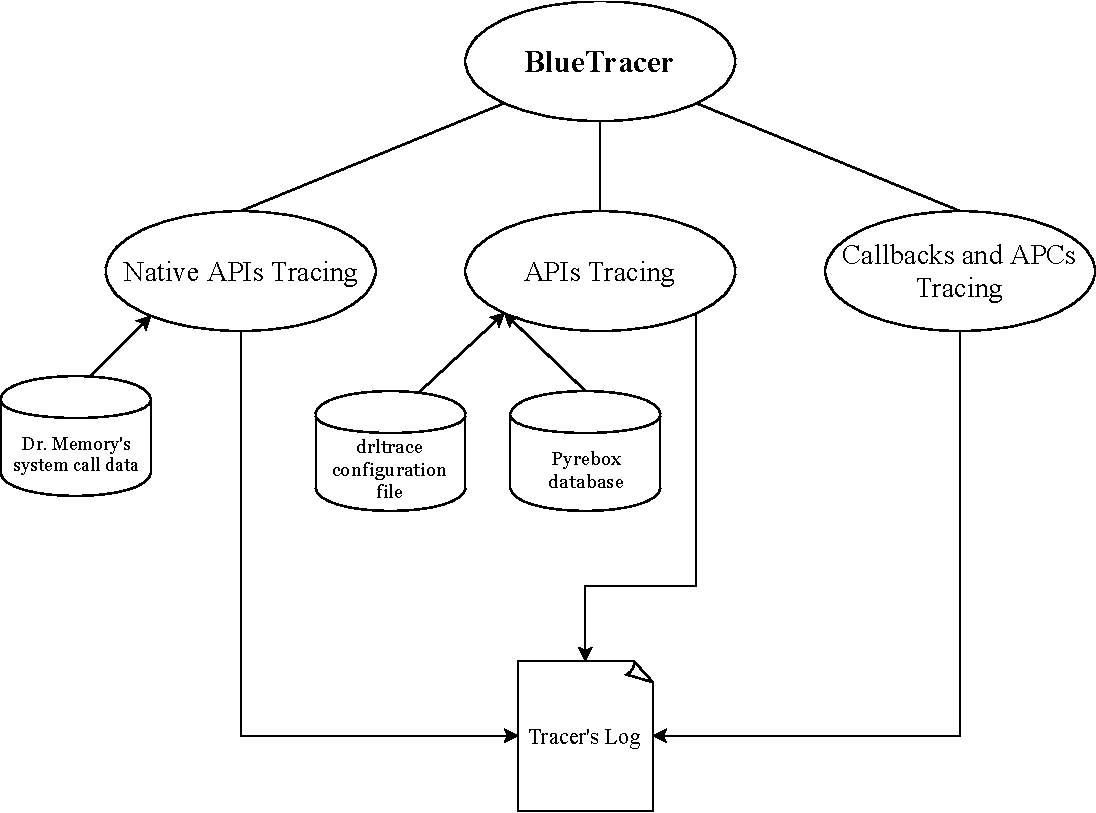
\includegraphics[scale=0.8]{Figures/BlueTracer.pdf}
\caption{\textit{BlueTracer's high level structure}}
\end{figure}

\section{Thread Management}

Since the samples under analysis are typically multithreaded applications, let us go through the mechanisms exposed by Pin to manage threads and how those were employed in the implementation of the tool.

Pin assigns to each thread an ID, a small number beginning at 0
which is not the same as the operating system thread ID. A way to obtain such ID is by using as analysis routine argument \texttt{IARG\_THREAD\_ID}, which passes the thread ID assigned by Pin for the calling thread. This ID is typically used as an index of an array of thread data.
In fact, the Pin API makes available an efficient thread local storage (TLS). In order to utilize it, it is first required to allocate a new TLS key via \texttt{PIN\_CreateThreadDataKey}, which can optionally take as input a pointer to a destructor function. After that, any thread of the process can use the TLS key, in addition to its Pin-specific thread ID, to store (\texttt{PIN\_SetThreadData}) and retrieve (\texttt{PIN\_GetThreadData}) values in its own slot. The starting value relative to the key in every thread is \texttt{NULL}.
Pin makes also available call-backs when each thread starts (registered with \texttt{PIN\_AddThreadStartFunction}) and ends (registered with \texttt{PIN\_AddThreadFiniFunction}). This is typically where thread local data is allocated, manipulated and stored in a thread's local storage\cite{Pin}.

In BlueTracer, each TLS slot stores a \texttt{struct} of the type \texttt{bluepill\_tls} (\textit{Listing 3.1}) for every thread. Such \texttt{struct} is dynamically allocated every time a thread starts in the \texttt{OnThreadStart} callback function and is consequently deallocated in the \texttt{onThreadFini} function when the thread ends.

\vspace{0.5cm}
\begin{lstlisting}[caption={Thread Local Data},captionpos=b]
typedef struct {
 ...
 syscall_tracer* syscallEntry;     // Pointer to NTAPI entry
 vector<stackEntry>* shadowStack;  // Shadow stack
 uint call_number;             	   // Calls counter							
 
 buf_info_t* buffer;		   	   // Buffer for writing to file				 
 FILE* OutFile;                    // Output file pointer
 
 // Pointer to function for opening file/writing to file	
 void(*file_write)(THREADID, buf_info_t*, FILE*, const char*, 	...);
 
 ...
} bluepill_tls;
\end{lstlisting}

Since the first three fields of the above \texttt{struct} (lines 3-5) are employed when tracing native APIs and APIs, they will be discussed in detail later in the chapter. Now let us focus on the remaining fields, which are used by BlueTracer to write the traced information in the appropriate log files. 

\subsection{Log Files and Multithreading}

In BlueTracer, the traced data is written to a binary file, one for every thread. The default naming convention used for the tracer's log files is \texttt{Traced.[OS Process ID].[Pin-specific Thread ID]}, similarly to the one Blue Pill employs in its own log files, with the user being able to change \texttt{Traced} with a name of its choice in the configuration file. 

When writing data to file, each thread invokes the \texttt{file\_write} function, whose pointer is located in the instance of the \texttt{bluepill\_tls} struct associated to the thread (line 11 of \textit{Listing 3.1}). However, such data, which follows the same format of strings used by \texttt{fprintf}, is not directly written to file. Instead, an intermediate 8 kB buffer is used (line 7 of \textit{Listing 3.1}): only when the buffer is full (or when the amount of data to be written does not fit the buffer) file writing actually occurs. The choice of using a buffer was made as an attempt to improve performance, as it allows the aggregation of small write operations into a block size that is more efficient for the disk subsystem.

A problem which was encountered when trying to conjugate file management and multithreading is that there exists a known isolation issue affecting Pin on Windows. Specifically, it is possible for a deadlock to take place if a file is opened in a callback in the context of multithreaded applications. As a result of this issue, it is not possible to open the tracer's log file in the \texttt{OnThreadStart} callback. Pin's manual proposes to circumvent the problem by opening the file in the \texttt{main} and tagging the data with the thread ID \cite{Pin}. However, this conflicts with the idea of having one file for each thread.

In order to bypass this limitation of the Pin's framework, the following strategy was employed:
\begin{enumerate}
\item When initializing the thread local data in \texttt{OnThreadStart}, \texttt{file\_write} is set to point to a function named \texttt{file\_open}.
\item The first time a thread attempts to write data to file \texttt{file\_open} is invoked.
\\
\\
\item \texttt{file\_open} carries out the following actions:
\begin{enumerate}
\item Opens the tracer's log file (this is safe since the file is not opened in a callback)
\item Sets the obtained file pointer in the thread local data (line 8 of \textit{Listing 3.1})
\item Adds the data to be written in the buffer (which is eventually written to file if the buffer is too small to hold it)
\item Sets \texttt{file\_write} to point to \texttt{buf\_write}, a function which is in charge of just writing data to the buffer and to file.
\end{enumerate}
\item As a result of this, when the thread attempts to write to file again, \texttt{buf\_write} is invoked, thus allowing the thread to just write to file without going through opening the file again.   
\end{enumerate}   

\section{Native APIs Tracing}
\iffalse
Talk about log structure when talking about how arguments are printed
\fi

Windows Native APIs are employed to call operating system services in kernel mode in a controlled way.  
In fact, all core Windows components, which possess direct access to hardware and services in charge of handling the computer's resources (e.g. memory), operate in kernel mode. This means that, every time a user mode application desires to carry out certain actions, like for instance starting a thread or allocating virtual memory, they must rely on kernel mode  services. The Windows Native API corresponds to the system call interface of standard monolithic operating systems, such as the majority of UNIX-like systems, with the difference that in the latter case the system call interface is documented and can be utilized directly by applications. Instead, due to Windows' architecture, Windows Native APIs are concealed to the programmer by the higher level Windows (\texttt{Win32}) APIs \cite{NTAPI1}. User mode Windows Native APIs, which are identified by their \texttt{Nt} prefix and are exported by \texttt{ntdll}, have caught the attention of malware writers since they are seen as a way of bypassing the documented APIs with the objective of performing a series of actions without being discovered \cite{NTAPI2}. For this reason it is a good idea to also trace them, in addition to the ordinary Windows APIs.  

Pin provides a set of APIs aimed at assisting the extraction of information relative to the system calls made by the pinned application, also including information relative to Windows Native APIs. In particular, in Blue Pill (and consequently in BlueTracer) \texttt{PIN\_AddSyscallEntryFunction} and  \texttt{PIN\_AddSyscallExitFunction} were used for this purpose. In fact, these allow to register notification functions which are called immediately before and after the execution of a system call \cite{Pin}. In BlueTracer, the function in charge of gathering Native API information before execution is \texttt{TraceSysCallEntry} while the one responsible for collecting Native API information after execution is \texttt{TraceSysCallExit}. They have been both been embedded in Blue Pill's notification functions and their overall structure is detailed in \textit{Figure 3.2}.
\\
\begin{figure}[h]
\centering
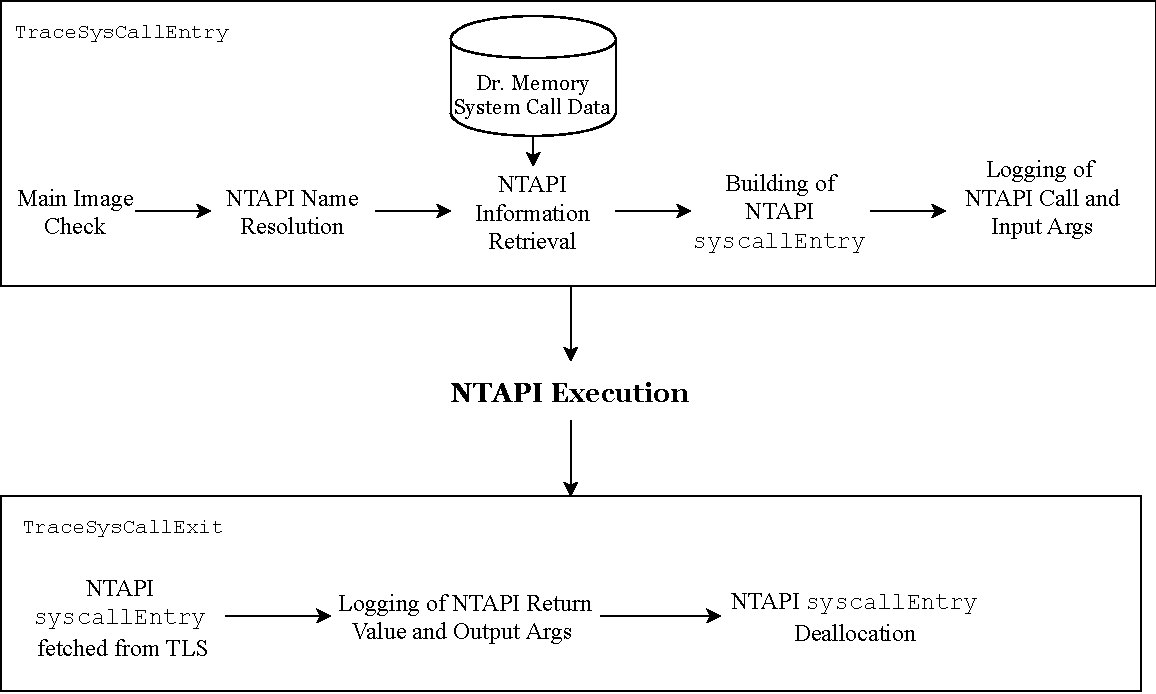
\includegraphics[scale=0.75]{Figures/NTAPITracing.pdf}
\caption{\textit{Native APIs Tracing Workflow}}
\end{figure}
\\
Following \textit{Figure 3.2}, let us now thoroughly analyze the main steps which take place when Native APIs are traced.

\subsection{Main Image Check}
\subsection{Native API Name Resolution}
\subsection{Native API Information Representation and Retrieval}
\subsection{Native API Logging}
Note: Include enum resolution here


\section{API}


\subsection{Shadow Stack}
\subsection{Performance}
\section{Callback and APC} 

\iffalse
\section{Tool Configuration}
\fi

\chapter{Experimental Results}

\chapter{Conclusions and Future Developments}

\printbibliography 


% Here put the code for the bibliography. You can use BibTeX or
% the BibLaTeX package or the simple environment thebibliography.
\end{document}